\section{Clasificación de segmentos VUS}

Se pide escribir función que para obtener el número de cruces por cero por milisegundo de una señal. El código escrito se muestra a continuación:
\begin{lstlisting}[language = octave]
function n_ms = cruces_zero(x,fs)
    n = 0;
    
    for i = 1:length(x)-1
        if x(i+1)*x(i) < 0
            n = n+1;
        end
    end
    
    ms = 1000*length(x)/fs;
    n_ms = n/ms;    
end
\end{lstlisting}

\subsection{Obtención de Criterios de Clasificación}

Para esta sección se utiliza el código \texttt{p2\_1.m}, el cual se adjunta a la entrega.

En primer primer lugar se separa la señal $training\_signal$ por cada letra con la ayuda del comando $ginput$. Esta señal corresponde a alguien diciendo ''señales temporales''. La separación se muestra en la figura \ref{fig:p2_1clas}
\begin{figure}[H]
    \centering
    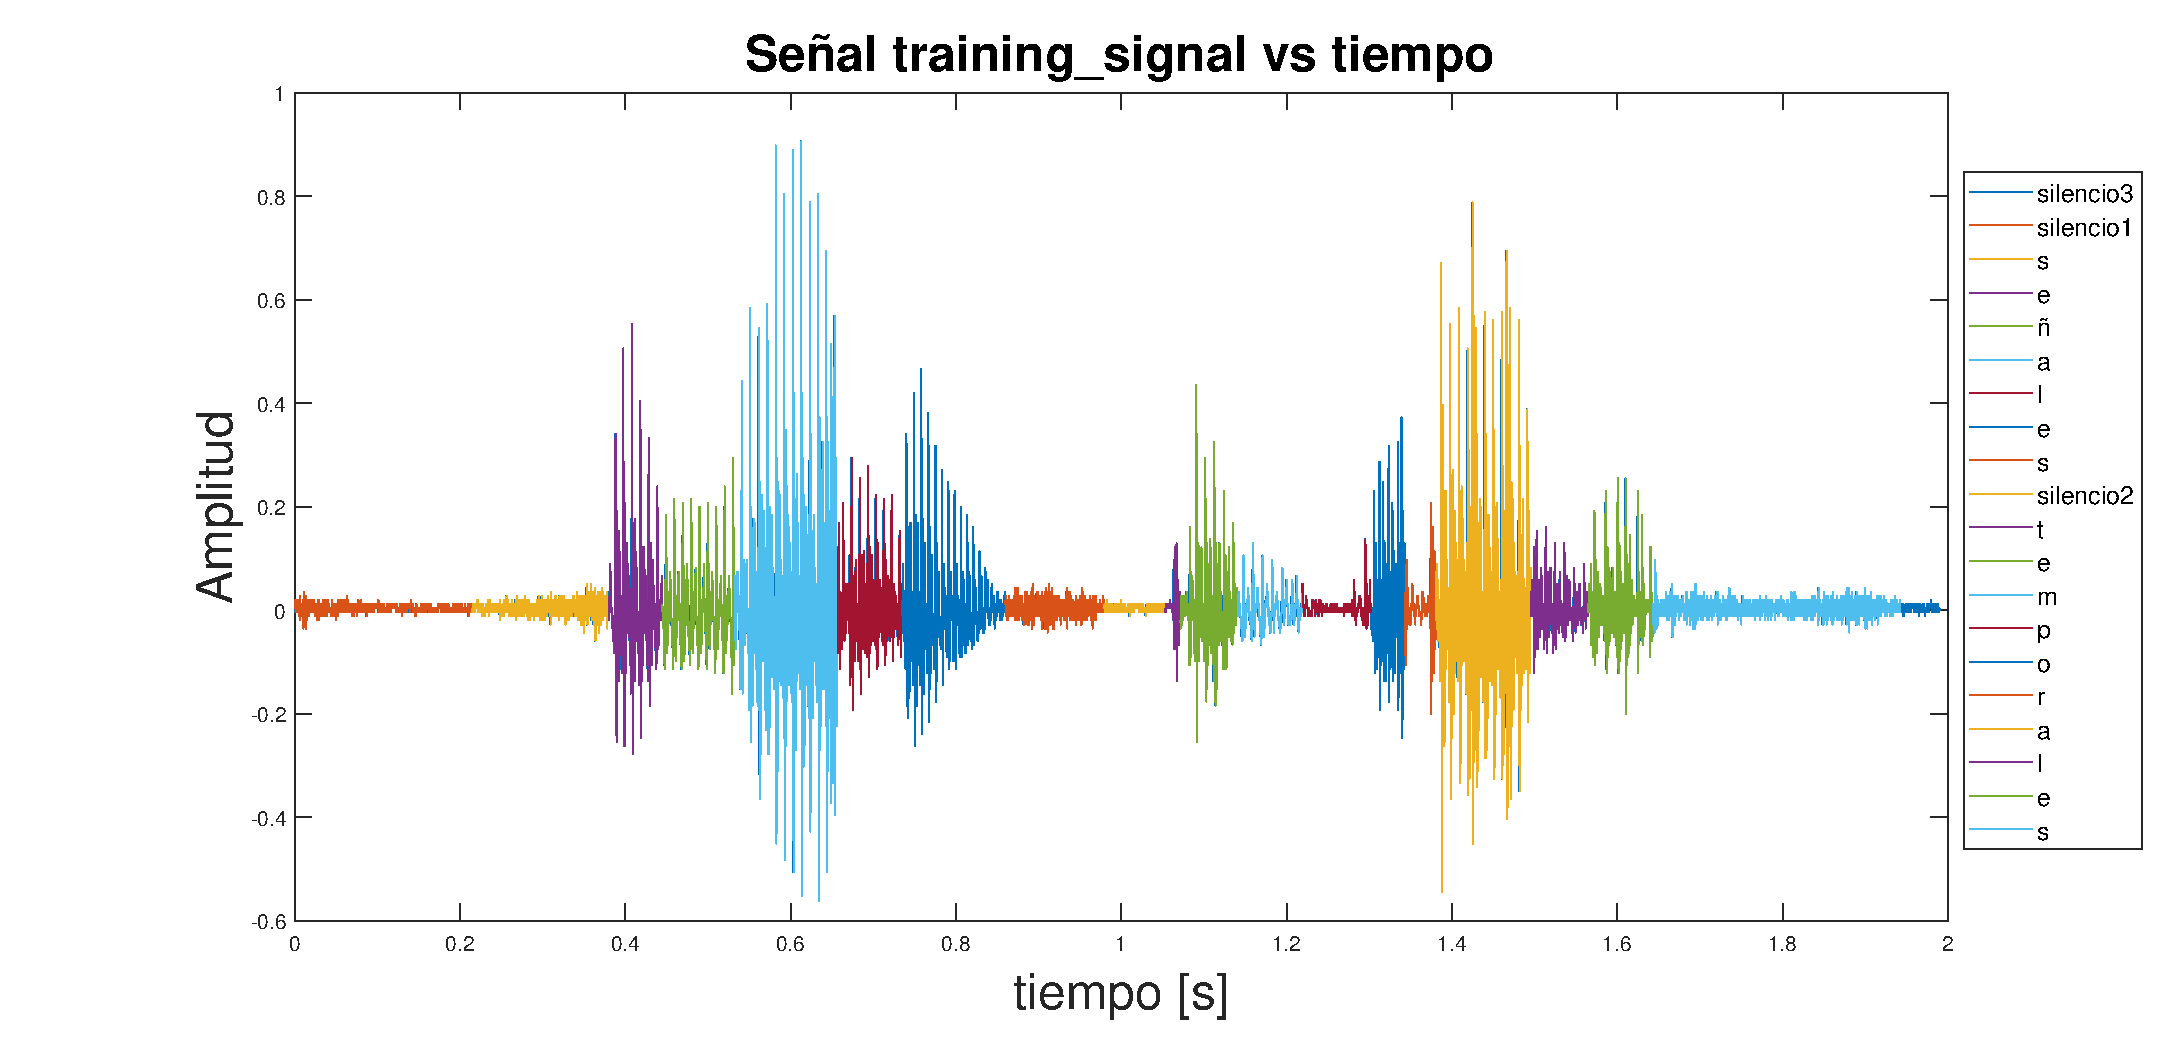
\includegraphics[width = .9\linewidth]{figures/p2_1separacion.eps}
    \caption{Separación manual por cada letra y silencios en señal $training\_signal$.}
    \label{fig:p2_1clas}
\end{figure}

En el cuadro \ref{tab:p2_1tab} se muestra el valor RMS, la razón de Cruces por Cero por milisegundo y la clasificación VUS de los segmentos encontrados en $training\_signal$.

\begin{table}[H]
    \centering
    \begin{tabular}{c|c|c|c}
        Sonido & RMS & Ratio Cruces por Cero & Clasificación VUS  \\ \hline
        Silencio 1    &0.0077     &2.7242 &S\\
        s             &0.0121     &3.8855 &U\\
        e             &0.0995     &1.6557 &V\\
        ñ             &0.0766     &1.0613 &U\\
        a             &0.1617     &2.9960 &V\\
        l             &0.0685     &2.3987 &U\\
        e             &0.0788     &1.5984 &V\\
        s             &0.0151     &4.5381 &U\\
        Silencio 2    &0.0061     &2.4678 &S\\
        t             &0.0359     &1.7297 &U\\
        e             &0.0714     &1.4756 &V\\
        m             &0.0336     &0.8166 &U\\
        p             &0.0161     &2.0000 &U\\
        o             &0.0911     &1.5181 &V\\
        r             &0.0394     &1.7627 &U\\
        a             &0.1525     &1.9349 &V\\
        l             &0.0412     &1.4611 &U\\
        e             &0.0544     &1.9904 &V\\
        s             &0.0136     &4.3554 &U\\
        Silencio 3    &0.0061     &2.4632 &S
    \end{tabular}
    \caption{Valor RMS, Ratio de Cruces por Cero por milisegundo y Clasificación VUS de segmentos encontrados en $training\_signal$}
    \label{tab:p2_1tab}
\end{table}

Posteriormente se obtiene una nube de puntos para los segmentos VUS, donde el eje horizontal corresponde al valor RMS y el vertical a los cruces por cero. Dicho gráfico se muestra en la figura \ref{fig:p2_1nube}.

\begin{figure}[H]
    \centering
    \includegraphics[width = .8\linewidth]{figures/p2_1nube.eps}
    \caption{Nube de puntos para los segmentos VUS para una posterior clasificación.}
    \label{fig:p2_1nube}
\end{figure}

A partir de la nube de puntos y una inspección visual sencilla se concluyen los siguientes criterios de clasificación:
\begin{enumerate}
    \item Valor RMS:
    \begin{itemize}
        \item Si $RMS < 0.01$: Sonido tipo S.
        \item Si $0.01 \leq RMS < 0.06$: Sonido tipo U.
        \item Si $RMS \geq 0.06$: Sonido tipo V.
    \end{itemize}
    
    \item Cruces por cero ($CZ$):
    \begin{itemize}
        \item Si $CZ < 2.25$: Sonido tipo V.
        \item Si $2.25 \leq CZ < 2.8$: Sonido tipo S.
        \item Si $CZ \geq 2.8$: Sonido tipo U.
    \end{itemize}
\end{enumerate}

Viendo la nube de puntos la decisión de clasificar los segmentos mediante umbrales en los cruces por cero no parece ser un método muy fiable. Por otro lado, umbrales en el valor RMS parece tener un mejor desempeño con respecto a la clasificación.

%%%%%%%%%%%%%%%%%%%%%%%%%%%%%%%%%%%%%%%%%%%%%%%%%%%%%%%%%%%5
\subsection{Comparación de criterios}

Para esta sección se utiliza el código \texttt{p2\_2.m}, el cual se adjunta a la entrega.

Cómo método combinado se propone:
\begin{enumerate}
    \item Valor RMS y Cruces por Cero ($CZ$):
    \begin{itemize}
        \item Si $CZ < -250RMS + 5$: Sonido tipo S.
        \item Si $CZ \geq -250RMS + 5$ y $RMS < 0.06$: Sonido tipo U.
        \item Si $RMS \geq 0.06$: Sonido tipo V.
    \end{itemize}
\end{enumerate}
El cual se obtuvo a partir de delimitar la nube de puntos obtenida en la sección anterior por 2 rectas, las cuales se muestran en la figura \ref{fig:p2_2nube}.

\begin{figure}[H]
    \centering
    \includegraphics[width = .8\linewidth]{figures/p2_2nube.eps}
    \caption{Nube de puntos para los segmentos VUS con rectas para clasificación con criterio combinado.}
    \label{fig:p2_2nube}
\end{figure}

Al revisar los resultados de los 3 métodos, se aprecia que:
\begin{itemize}
    \item El criterio de los Cruces por Cero presenta resultados no satisfactorios. Lo anterior era esperable debido a que no se apreciaba una correlación en la nube de puntos lo suficientemente fuerte como para aplicar umbrales.
    \item El criterio del valor RMS presenta resultados bastante mejores que el de cruces por cero. De la nube de puntos era esperable que umbrales en el valor RMS (separación del plano por líneas verticales) debía dar mejores resultados en la clasificación.
    \item El criterio combinado propuesto entrega resultados muy similares de clasificación de puntos. Lo anterior no es una sorpresa, ya que este criterio puede interpretarse como una leve inclinación de la recta vertical correspondiente al umbral más bajo del criterio RMS.
\end{itemize}

Por todo lo anterior se concluye que desde una perspectiva costo-efectivo el mejor criterio encontrado corresponde al del valor RMS. 

%Debiese haber un parrafo donde propongas el método combinado (puede ser también por umbrales y alguna combinación lineal). Con que sea al ojo cualquier cosa mas o menos lógica está bien. Te puedes justificar en función a la nube de puntos de la figura p2_1nube

% Tienes que implementar el método en matlab. usa umbrales nomás y sera copiar y pegar código que ya está en el p2_2.m.

%Tiene que haber un segundo párrafo donde comentes como anduvieron estos 3 métodos. El de cruces por cero es re malo así que al final será comparar el RMS con el propuesto por tí y probablemente se concluya que el mejor en terminos costo-efectividad sea el criterio RMS.


%%%%%%
Finalmente se grafica la señal $text\_signal$, la variable VUS (1, -1 o 0) obtenida a partir de la estimación de RMS y el valor RMS de los segmentos. Dichos gráficos se muestran en la figura \ref{fig:p2_2grafs}. Con respecto a los gráficos se puede comentar que:
\begin{itemize}
    \item Como es de esperarse, el valor RMS se comporta como una especie de envolvente de la señal.
    \item Al ser la señal ''sonidos de voz'' es claro que el criterio presenta falencias en la clasificación.
    \item A partir de la evolución del valor RMS en el tiempo, podría mejorar la clasificación cambiando los umbrales.
\end{itemize}

\begin{figure}[H]
    \centering
    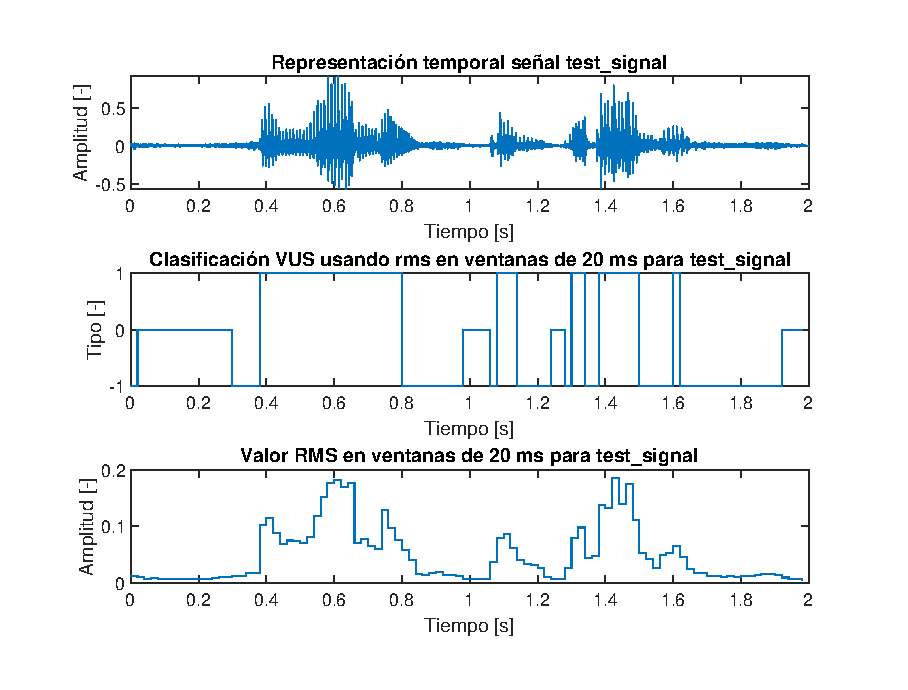
\includegraphics[width = .9\linewidth]{figures/p2_2grafs.eps}
    \caption{Señal $text\_signal$, clasificación VUS (RMS) y valor RMS de segmentos clasificados.}
    \label{fig:p2_2grafs}
\end{figure}







